\chapter{Technologies}
%Describe here Vuforia, OpenCV, FastCV, UIKit, etc.
Ponster is an augmented reality app developed for the iOS platform. In order to make
possible all the features that enable us to try the poster images in the camera
scene, two main technologies have been used. First of all, the iOS SDK provided by
Apple\textregistered ~is needed to develop any iOS application. For the augmented reality, OpenCV
has been the first SDK tested, but finally the Vuforia SDK\cite{vuforia} developed
by Qualcomm\textregistered ~has been the one used in Ponster. We will start this
discussing first the iOS SDK, and then the augmented reality technologies used.

\section{iOS}
The Apple iOS SDK has been used to develop the native, augmented reality
application. The development started using the 7.1 version and the final release has
been made with the latest SDK version, iOS 8. Several frameworks have been used to
enable us to show the posters with a waterfall layout, fetch the data of the posters
from the local database and to get input from the camera of the device.

The most important frameworks used are described in the next sections, and include
UIKit, CoreData and other third party libraries.

\subsection{UIKit}
UIKit\cite{uikit} is Apple's framework to build iOS interfaces both in iPad and
iPhone devices. All of the UIKit's classes inherit from a common interface object
called \texttt{NSObject}. This framework provides classes to manage gestures, fonts,
navigation bars, tab bars, text inputs, images, tables, buttons and many more
elements. Almost every iOS application uses UIKit in one way or another. Only some
videogames do not make extensive use of the framework due to the specific user
interfaces and game engines that most of them use. 

Most of the Apple's frameworks naming convention date back from the NeXTStep era. They're written in
Objective-C and they use the two-letter class prefix in all of them, making easy to
identify to which framework belongs each class. For instance, all the UIKit classes
have the \texttt{UI} class prefix. \texttt{UITextField} or \texttt{UIView} both
belong to UIKit. In other hand, \texttt{NSObject}, which belongs to Foundation
framework, has the NeXTStep NS prefix.

In Ponster several UIKit features have been used. For the main user interface, a
navigation-based UI is provided by \texttt{UINavigationController}. The main screen
of Ponster shows a \texttt{UICollectionViewLayout} interface with a custom waterfall
layout. This layout enables us to fit images with different sizes preserving their
aspect ratio. Each image represents a subclass of \texttt{UICollectionViewCell} with
custom elements, such as a \texttt{UIImageView} for the poster and a \texttt{UILabel}
for it's title. In the image
\ref{fig:iosapp01} we can see an example of the navigation-based interface of
Ponster and the collection view layout.

\begin{figure}
\centering
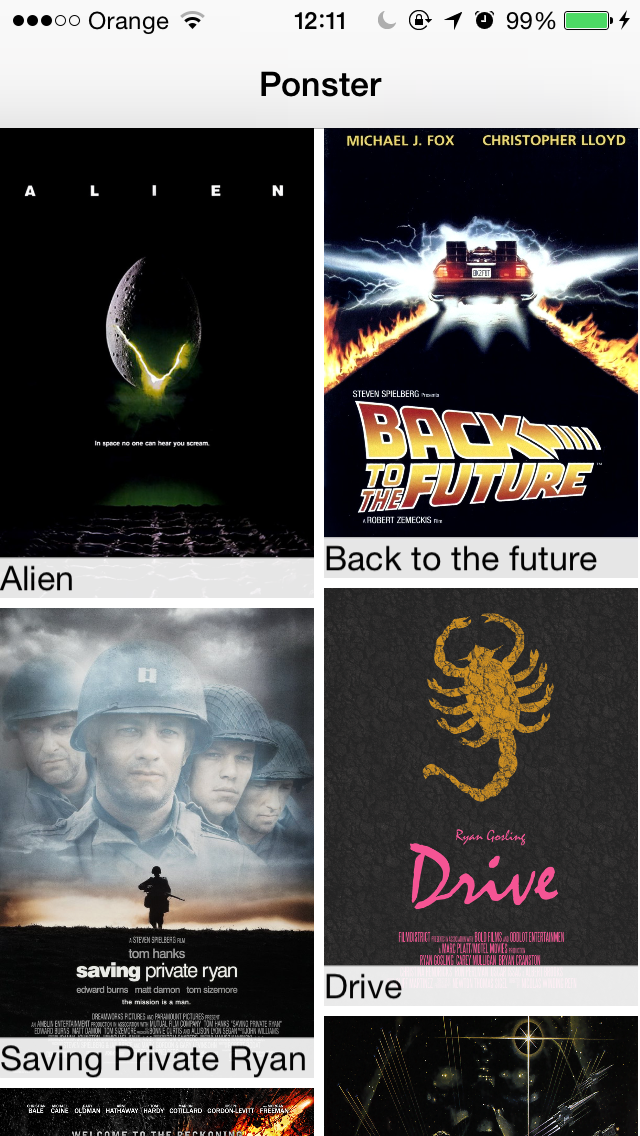
\includegraphics[scale=0.35]{img/iosapp01.png}
\caption{\label{fig:iosapp01}Main interface of Ponster demonstrating the use of
  navigation controllers and collection layouts.}
\end{figure} 

Other UIKit features used in Ponster include \texttt{UIButton}s, \texttt{UISwitch}
and \texttt{UIGestureRecognizer}s. 

\subsection{CoreData, persistence layer for iOS applications}
The main purpose of the research presented in the chapter \ref{chap:sota} was to
bring augmented reality to display posters in any surface the user wants
to. However, Ponster app has been developed with the addition of more features in
mind. One of this features is data persistency.

In order to mantain a list of all the posters included in the app --they are bundled
inside the app in this version--, we have several methods to include and display
this information. The simplest option is to save the data in the preferences
\texttt{.plist} file and then read all the values. Also, we could use
\texttt{NSKeyedArchiver} to save data from our object model into the application
sandbox. But, the best way to maintain data and to
query it from our application is to use a real SQL database. CoreData integrates
the SQLite database with a class-based model approach that enables us to save and
retrieve information easily.

With the CoreData framework, we design an object model (figure~\ref{fig:coredata}) and then we
generate the model classes. Each class is a subclass of \texttt{NSManagedObject}
that has all the attributes that we've added in our model. Inside the application,
we can query or model by class, and then retrieve the objects as an array. Each
model object is like any other object, and we can access to it's properties using
the common dot notation. For example, we can access to the \texttt{imageUrl}
property in the following way:

\begin{verbatim}
Poster *poster = (Poster *)item;
UIImage *posterImage = [UIImage imageNamed:poster.imageUrl];
\end{verbatim}

\begin{figure}
\centering
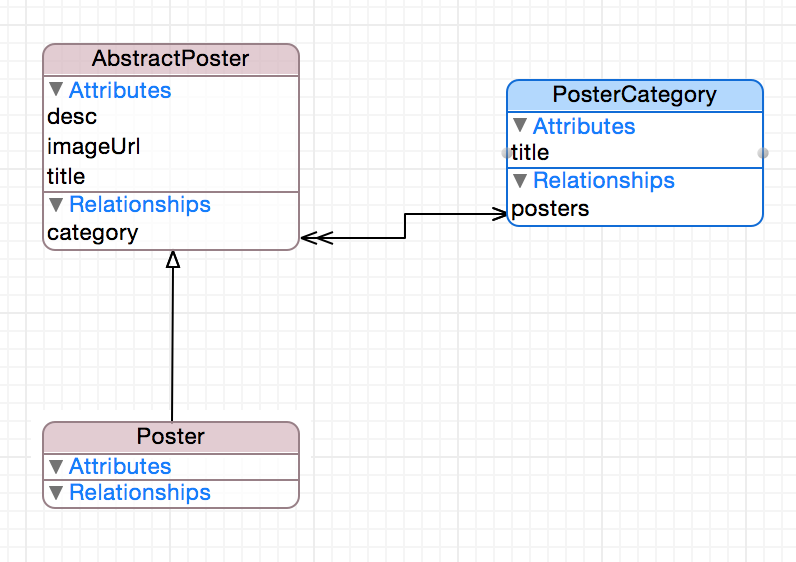
\includegraphics[scale=0.65]{img/coredata.png}
\caption{\label{fig:coredata}Basic data model of Ponster. The CoreData model editor
  enables us to design the model and then generate all the object classes. The
  double arrow represents a to-many relationship and the white arrow represents
  object inheritance.}
\end{figure} 

CoreData's stack enables us to perform queries and to save information in the SQLite
store. Due to the fact that iOS applications use a maximum-priority thread for the
UI calculations, and several other threads with lower priority to perform other
tasks, it's fundamental to understand how CoreData performs it's operations and how
can we use it efficiently. In the section~\ref{sec:architecture}, our CoreData
architecture is presented.

Three objects are fundamental to CoreData, the \textbf{context}, the \textbf{coordinator}
and the \textbf{store}. The \texttt{NSManagedObject\textbf{Context}} is used to perform
any save or query operation to the CoreData stack. The
\texttt{NSPersistentStore\textbf{Coordinator}} is the object that communicates
between the contexts and the stores. Finally, the
\texttt{NSPersistent\textbf{Store}} is the responsable of applying the changes to
the SQLite backend. The store and the coordinator are initialized once you start
your app. All the data that we've saved is present in the SQLite file, inside our
application sandbox. Apps can use more than one context, as we discuss
in~\ref{sec:architecture}, and every operation against the database must be
performed in a context. For example, when we want to perform a request for a
selected \textit{entity}, we have to specify the context:

\begin{verbatim}
NSFetchRequest *request = [[NSFetchRequest alloc] init];
NSEntityDescription *entityDescription = [NSEntityDescription
entityForName:entityName inManagedObjectContext:context];
[request setEntity:entityDescription];
// Build and perform the query
[request setPredicate:...];
\end{verbatim}

Finally, CoreData works very well with another important class,
\texttt{NSFetchedResultsController}. This class allows us to watch for changes in
any class in our model, with any predicate we want, thus performing an automatic
refresh of our data every time some change in our model has been done in the
monitorized classes. The fetched results controller is the class that comunicates
our view controllers with the data model.

\subsection{AVFoundation}
AVFoundation is used in Ponster to get the images from the camera of the device. A
\texttt{AVCaptureVideoDataOutput} can be configured to get the frames of the
camera. This output can be configured to deliver an specific amount of frames per
second, the pixel format of the output or the orientation of the camera. Each of the
frames delivered by the \texttt{AVCaptureVideoDataOutputSampleBufferDelegate} is
sent to the augmented reality algorithm to perform the matching.

\subsection{Third-party libraries}
Several third-party libraries are used in Ponster. One of them is the OpenCV SDK and
Vuforia SDK, which we're going to discuss in the next section. The other two
interesting libraries are \textbf{MagicalRecord} and
\textbf{PDKTCollectionViewWaterfallLayout}, along with the package dependency
manager \textbf{CocoaPods}.

\begin{description}
\item [MagicalRecord] \hfill \\
MagicalRecord\ref{gh:mr} is a library written by Saul Mora that makes easy to use
CoreData. It acts as a wrapper for most of the CoreData's actions and makes possible
to perform any action with less lines. Also, MagicalRecord helps us to create new
contexts, which is very important in our application architecture.
\item [PDKTCollectionViewWaterfallLayout] \hfill \\
PDKTCollectionViewWaterfallLayout is a \texttt{UICollectionViewLayout} that enables
us to organize the cells of the collection view in a waterfall-style layout. With
this we can display different cell sizes by preserving their aspect ratio and
maintaining the same width.
\end{description}

\subsubsection{CocoaPods dependency manager}
This two third-party libraries, along with OpenCV, have been installed and added to
Ponster by using CocoaPods. CocoaPods is the dependency manager for Objective-C
projects\cite{cocoapods}. It is an open-source project sponsored by several
companies that it's becoming very popular among iOS and Mac developers.

With CocoaPods it is easy for developers to generate a \texttt{Podspec} for their
projects and share them with the community. For instance, an iOS OpenCV compilation
is maintained by several developers and they have recently added a Podspec --a small
file with the description of the version of the project, the repository of the
source code and their dependencies-- to make easier to integrate OpenCV in iOS
projects. With CocoaPods we just have to create a \texttt{Podfile} with all the
dependencies we want to install, and then by just entering \texttt{pod install} in
the project directory, all the dependencies are installed and linked as a
subproject.

This dependency manager allows developers to easily add or remove dependencies to
their projects, and also makes easy to share their libraries with others. CocoaPods
is distributed as a Ruby gem and it can be installed easily in any Mac computer.

\section{Computer vision}
Two computer vision libraries have been used, OpenCV in the first stages of
development, and later Vuforia, which is made by Qualcomm\textregistered. 

\subsection{OpenCV}
\subsection{Vuforia}
\subsubsection{FastCV}
